\documentclass[a4paper,11pt]{report}

\usepackage{rathaxesmmix}
\usepackage{graphicx}
%---------------------------------------------------------


\title{Rathaxes technical documentation}
\author{David Giron, Adrien Silvestre, Vivien Jacquemmoz - Rathaxes}
\date{Thursday May 29th 2008}


\begin{document}
  \maketitle


%---------------------------------------------------------


  \section*{License}
  \addcontentsline{toc}{section}{License}
  Copyright (c) 2007 Rathaxes Team (team@rathaxes.eu)
  \\\\
  Permission to use, copy, modify, and distribute this software for any
  purpose with or without fee is hereby granted, provided that the above
  copyright notice and this permission notice appear in all copies.
  \\\\
  THE ARTICLE IS PROVIDED "AS IS" AND THE AUTHOR DISCLAIMS ALL WARRANTIES
  WITH REGARD TO THIS ARTICLE INCLUDING ALL IMPLIED WARRANTIES OF
  MERCHANTABILITY AND FITNESS. IN NO EVENT SHALL THE AUTHOR BE LIABLE FOR
  ANY SPECIAL, DIRECT, INDIRECT, OR CONSEQUENTIAL DAMAGES OR ANY DAMAGES
  WHATSOEVER RESULTING FROM LOSS OF USE, DATA OR PROFITS, WHETHER IN AN
  ACTION OF CONTRACT, NEGLIGENCE OR OTHER TORTUOUS ACTION, ARISING OUT OF
  OR IN CONNECTION WITH THE USE OR PERFORMANCE OF THIS SOFTWARE.
  \newpage


%---------------------------------------------------------


  \section*{Introduction}
  \addcontentsline{toc}{section}{Introduction}
  Welcome to Rathaxes, the open source, Driver generator. Powered by pure Rhino.
  The goal of the project is to provide an innovative language approach to driver
  developpement. A simple descriptive DSL to encapsulate all of the comportments
  of a device driver on any Operating System (just four of them for the moment)
  Robustness, portability and modularity, that's what the Rathaxes compiler is
  built for.

  \chapter{CodeWorker}
  CodeWorker is an Open Source parsing tool and a source code generator devoted
  to generative programming made by Cedrick Lemaire. Generative programming is
  a software engineering approach interested in automating the production of
  reusable, tailor-made, adaptable and reliable IT systems.
  In layman's terms, CodeWorker lets you generate code by parsing existing
  languages, or by creating and parsing your own language. We will be using it
  for this exact purpose as ``a compiler of compilers''. Once a language file
  has been parsed, CodeWorker provides several techniques for generating code.
  \\
  The tool's scripting language drives the parsing and source code generation
  process.Its syntax is derived from the C family of languages, making it
  familiar to most programmers. The template syntax is like JSP, ASP, or
  Velocity. It has variations for parsing, code generation, or procedural
  programming, giving the developer a number of options for organizing
  CodeWorker projects. 
  \\
  Codeworker is more powerful and easier to use than Lex/Yacc, CodeWorker is
  perfectly fits Rathaxes' code generation needs. It can be divided into three
  major parts:

  \begin{itemize}
    \item BNF description langage: Codeworker's parsing language requires a
      simple BNF description of the language to parse. The RDSL and the BDSL
      of Rathaxes will be described thus.
    \item Scripting langage: Codeworker scripts are powerful enough for the tree
      decoration needs of Rathaxes.
    \item generation scripting langage: We will then use the templating
      functionalities of Codeworker to generate C code.
  \end{itemize}

  \chapter{Cnorm}
  Cnorm is a C parsing tool written with CodeWorker made by Lionel Auroux
  (Epita/Epitech system \& security labotory's boss), Cedrick Lemaire
  (CodeWorker's developper) and David Giron, David Amsallem and Christophe
  Fajardo (all from the Rathaxes team).

  This parser has been designed to be as powerful as possible to be able to
  parse both the C-Unix and C-Windows codes.
   
  \begin{itemize}
   \item Standard C 89 syntax
   \item GnuC asm expression
   \item GnuC \_\_thread storage class specifier
   \item GnuC parameter forward declaration
   \item GnuC \_\_extension\_\_ evite les warnings sur l'utilisation d'extention
     GnuC
   \item GnuC subscript
   \item GnuC designated initializer
   \item GnuC \_\_builtin\_offsetof
   \item GnuC \_\_builtin\_va\_list
   \item c99 static in direct absolute declarator
   \item c99 block as single expression (\{ \})
   \item c99 typeof
   \item c99 designation
   \item c99 \_\_alignof
   \item c99 complex,\_\_real \& \_\_imag operator
   \item c99 range expression
   \item c99 and Windows attributes
   \item K. \& R. coding style
   \item Missing type in function declaration
  \end{itemize}

   This grammar was adapted from the one in section A13 of the C programming
   language, second edition, by Brian W. Kernighan and Dennis M. Ritchie
   (Englewood Cliffs, New Jersey: Prentice Hall PTR, 1988; ISBN 0-13-110362-8),
   pages 234 - 238. 
   \\
   Cnorm is used in Rathaxes to parse the C code present in the BDSL in order to
   avoid opaque datas and to provide full control on the handled code.
   The C abstract syntax tree organisation ca be found in Cnorm's own
   documentation. It won't be covered by this one.

  \chapter{Functional description}
  
    \section{Functional diagram}
    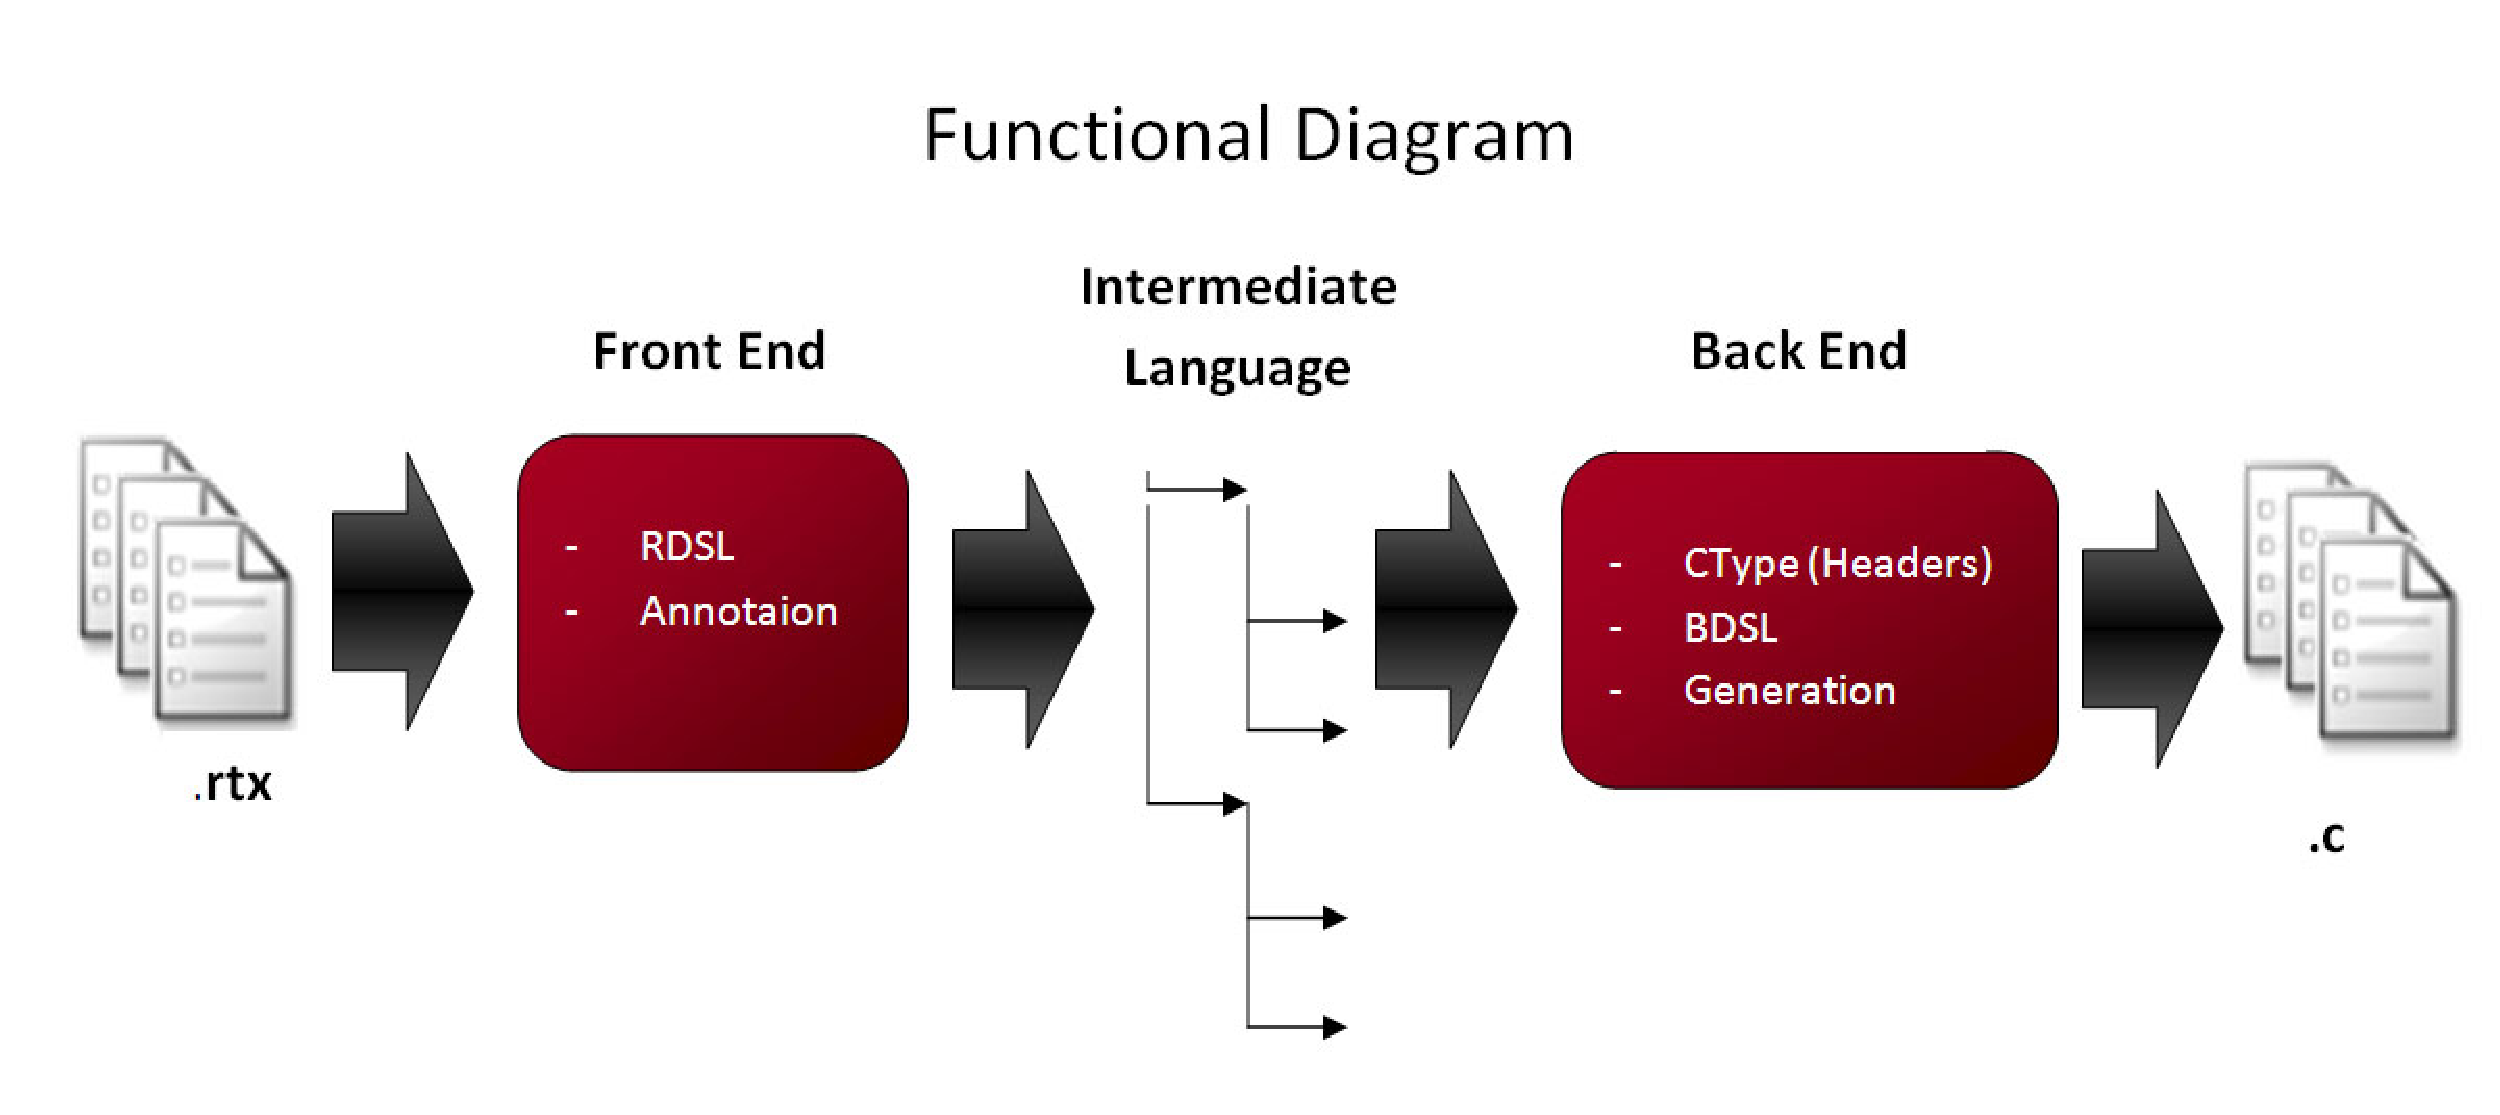
\includegraphics[width=13cm]{functional_diagram}

    \section{Compiler anatomy}
    The Rathaxes compiler follows the most classical architecture for compilers.
    It is built with a Front End dedicated to translating the source code into
    an abstract syntax tree exploitable by the program; and a back end  that
    will use this tree to generate the target code through a large library of
    dynamic templates.
    \\
    Its inner workings can be functionally divided in five main parts :
    \begin{itemize}
     \item RDSL parsing:\\
       Ok, so we wanna generate a fully functional driver. The first step in
       rathaxes is parsing our RDSL, the language in which the driver is
       described, and turn that into a preliminary tree. The language will be
       described a bit further on.
     \item Abstract Syntax Tree decoration:\\
       Second step, our tree doesn't contain enough information yet. We will now
       use scripts to decorate it, adding information where it is necessary.
     \item BDSL templates harvesting:\\
       Our templates are not static pieces of code to be inserted 'as is' inside
       the generated code. The templates are stocked into .blt (black library
       templates) files and are parsed during execution. The templates
       themselves are written in an aspectual templating language, that allow
       the description of a complex set of conditional rules for the generated
       code. These templates will be parsed and translated into an independant
       data tree. It is important to note that there for the moment there are no
       "direct copy" directives in Rathaxes. Everything is parsed, even the C
       code. So your templates will will have to compile, your system types will
       have to be correct. The c trees are generated through the Cnorm tool that
       we have talked about before. It is important to note also that for the
       moment it is still possible to call codeworker scripts directly from the
       templates.
     \item Linking:\\
       So, we've got two trees, one containing the parsed data from the input
       file and the other one containing the parsed data from the templates.
       We now have a step of linking to "fuse" the two trees into one. We'll use
       various scripts to make our final tree in which the flags activated
       during frontal parsing will be linked to the aspects met in the templates.
     \item Generation:\\
       We now have everything we need to generate our target code. One last
       Codeworker script to explore the tree, and write the C code. We're using
       another external tool for this, the pretty printer, which generates C from
       a C AST generated by Cnorm.
    \end{itemize}



    \section{Rathaxes' frontend}

      \subsection{RDSL Parsing}
	Rathaxes is a compiler and as such it first has to parse source code.
        Our source code is written in RDSL (Yeah I know lame name, but we're
        looking for a better one) A descriptive language dedicated to describing
        generically device drivers.
        \\
	There are two main concepts inside the DSL :

        \begin{itemize}
          \item The device block which is used as a physical description of the device. It includes 
	    Description of the core behavior of the device. Its physical interfaces (registers), its data 
	    treatment (algorithms)
          \item The driver block: which is used as ``configuration for the pointed device'' it includes 
	    Implementation of the driver syscalls IRQs stuff like that.
        \end{itemize}

	A very important part of Rathaxes is the semantic division of device drivers. Pay attention because 
	nearly all of the concepts behind Rathaxes rely on this model. The Rathaxes research team has worked
	hard, and has invented a modelisation of device drivers that divide their core components into 
	into seven main parts, semantically distinct and significant.
	These 'semantics' are essential in the description of the drivers Rathaxes uses.
        \begin{itemize}
          \item LKM\\
		The first layer : Loadable kernel modules. How do you add code in your kernel ? You have two 
		solutions, you can recompile it, extremely annoying solution, major time waster. Or you could
		simply add a module inside your kernel This semantic encapsulates all the interactions
		 and the data needed to add a module in the target kernel. These semantics are encapsulated in 
		the device and driver blocks.
          \item userland interface\\
	  	This layer contains the functions the user will interact with in the normal use of the device,
		 such as read,write and IOCTL. these semantics are encaspulated in the Userland blocks.
          \item lib/bus\\
	        This layer contains the necessary data and function to  Resolve communication from hardware 
		to CPU through the different bus libraries	
          \item callback\\
	  	This layer is used to let the drivers register the different callbacks it will need to use
		during its use. Like IRQs and such.
          \item io\\
                Direct Communication between the CPU and the hardware through In and out instructions. 
          \item register\\ 
	        Data is stored and is accessible inside electronic components through registers. 
		Rathaxes offers an abstraction layer over theses registers, for simplification and error 
		reduction purose. The Register layer encapsulates the way these registers work and such.
		All of that inside the Register blocks.
          \item algorithm\\
                And finally the data will have to be treated before it can be of any use to the kernel.
		The last layer encapsulates thess algorithms.
       \end{itemize}
      \subsection{Tree decoration}
	We have now parsed the source code, and we've got an abstract syntaxic tree that is a direct representation
	of it. It is far from being complete yet. We are now going to decorate it according to our needs. As
	we've explained higher, every syntaxic block in Rathaxes belongs to one of the driver semantics we've defined.
	First we'll go through our tree to activate the semantics in the semantics table. Then we'll have to dispatch
	the harvested data in the tree according to the semantics. 
	In this step we'll also have to activate the sub-semantics, but we're not completely done implementing that. 

    \section{Rathaxes' backend}

      \subsection{Black Library Templates}
	
	Rathaxes is a compiler, it generates Code. And as such it needs a large library of templates to generate code. 
	We call it ''the black library''. It is extremely important to understand that Rathaxes' templates are not static
	piece of codes that will be recopied directly in the target file.
	
	Our templates are written in an aspectual templating dsl that allows modularity of the generated code. The 
	aspectual paradigm is represented by a collection of Advices and Joinpoints that are 'activated' according
	to the semantics flags we have mentioned earlier. First each target operating system must have a personal 
	directory in the root directory of the Black library. In this directory the real templates will be organised into
        by OS, each one in a directory going by the exact name of the OS. Inside this Os directory we will have seven
	main sub-directories one for each driver semantics. these will contain the templates in themselves, each one
	independantly representing its inner data through a tree of aspectual templates.
	Secondly we'll have in this directory, a tree of dependencies between the different header files of the
	operating system, and a cache of the system types. The first part is extremely important in some operating system
	who forbid to include files, inside a file that will be included. Therefore includes must be done in a certain
	order. The second part is essential to rathaxes. As I've said earlier all of our templates are parsed and 
	translated into a tree. Everything, even the c code is parsed through the Cnorm tool. The code needs to compile
	for it to be accepted by rathaxes. We therefore need to know every system types for the code to compile. We 
	could reparse every kernel header each time we compile a new driver, but that tends to take rather a long 
	time, about 30 seconds a compilation from our experience. We therefore found a solution of caching the 
	system types into associative tables because those are the only real informations needed for compilation. 	 
       	We will someday include compilation script generators.

        The templates in themseleves, are written inside Our aspectual DSL. But for the moment we can still call
	codeWorker scripts. We intend to discourage that as the project develops. But for the moment it can be 
	used to store variables, to call functions, to treat data... Then we've got our DSL itself. We have developped
	it as a tool to describe, easily modular templates. It allows insertion relevant code anywhere during 
	the generation process, according to different conditional flags activated during the parsing of the RDSL.
	The flags are representation of the main driver semantics and their sub-semantics. And of coures you've got 
	the C code, encapsulated by all the elements we've talked above.  C has been for many years the most common
        language of device driver developpement. as such it is human readable, portable and adaptable.
	
      \subsection{Aspect selection (linking)}
	
	To sum up, we now have two separate trees, the source code, and the templates. We now have to fuse these two 
	trees, in  a shape that will be a direct representation of the code we endeavour to generate. First step is 
	to resolve the activated Joinpoints inside our tree, and of the advices. We'll also resolve the notions of
	before, after and around absolutely essential to the aspectual paradigm. Some of it is not implemented yet. 
	Right now the black library is still more like a recipe, with a beginning point, which describes a path
	from  the beginning of the compiling to a typical end with optional branches activated by the semantic flags.
	We are working to change that, to switch the burden of piloting the compiler from the template library to the
	source code, and to let the black library be a simple container of possible 'ingredients'

      \subsection{Generation}
	Still with us ? We now have everything we need for generation. We are going to pass our tree to the PrettyPrinter
	an external tool that takes parsed C and translates it into C.

  \chapter{Implementation Description}

    \section{Implementation diagram}
    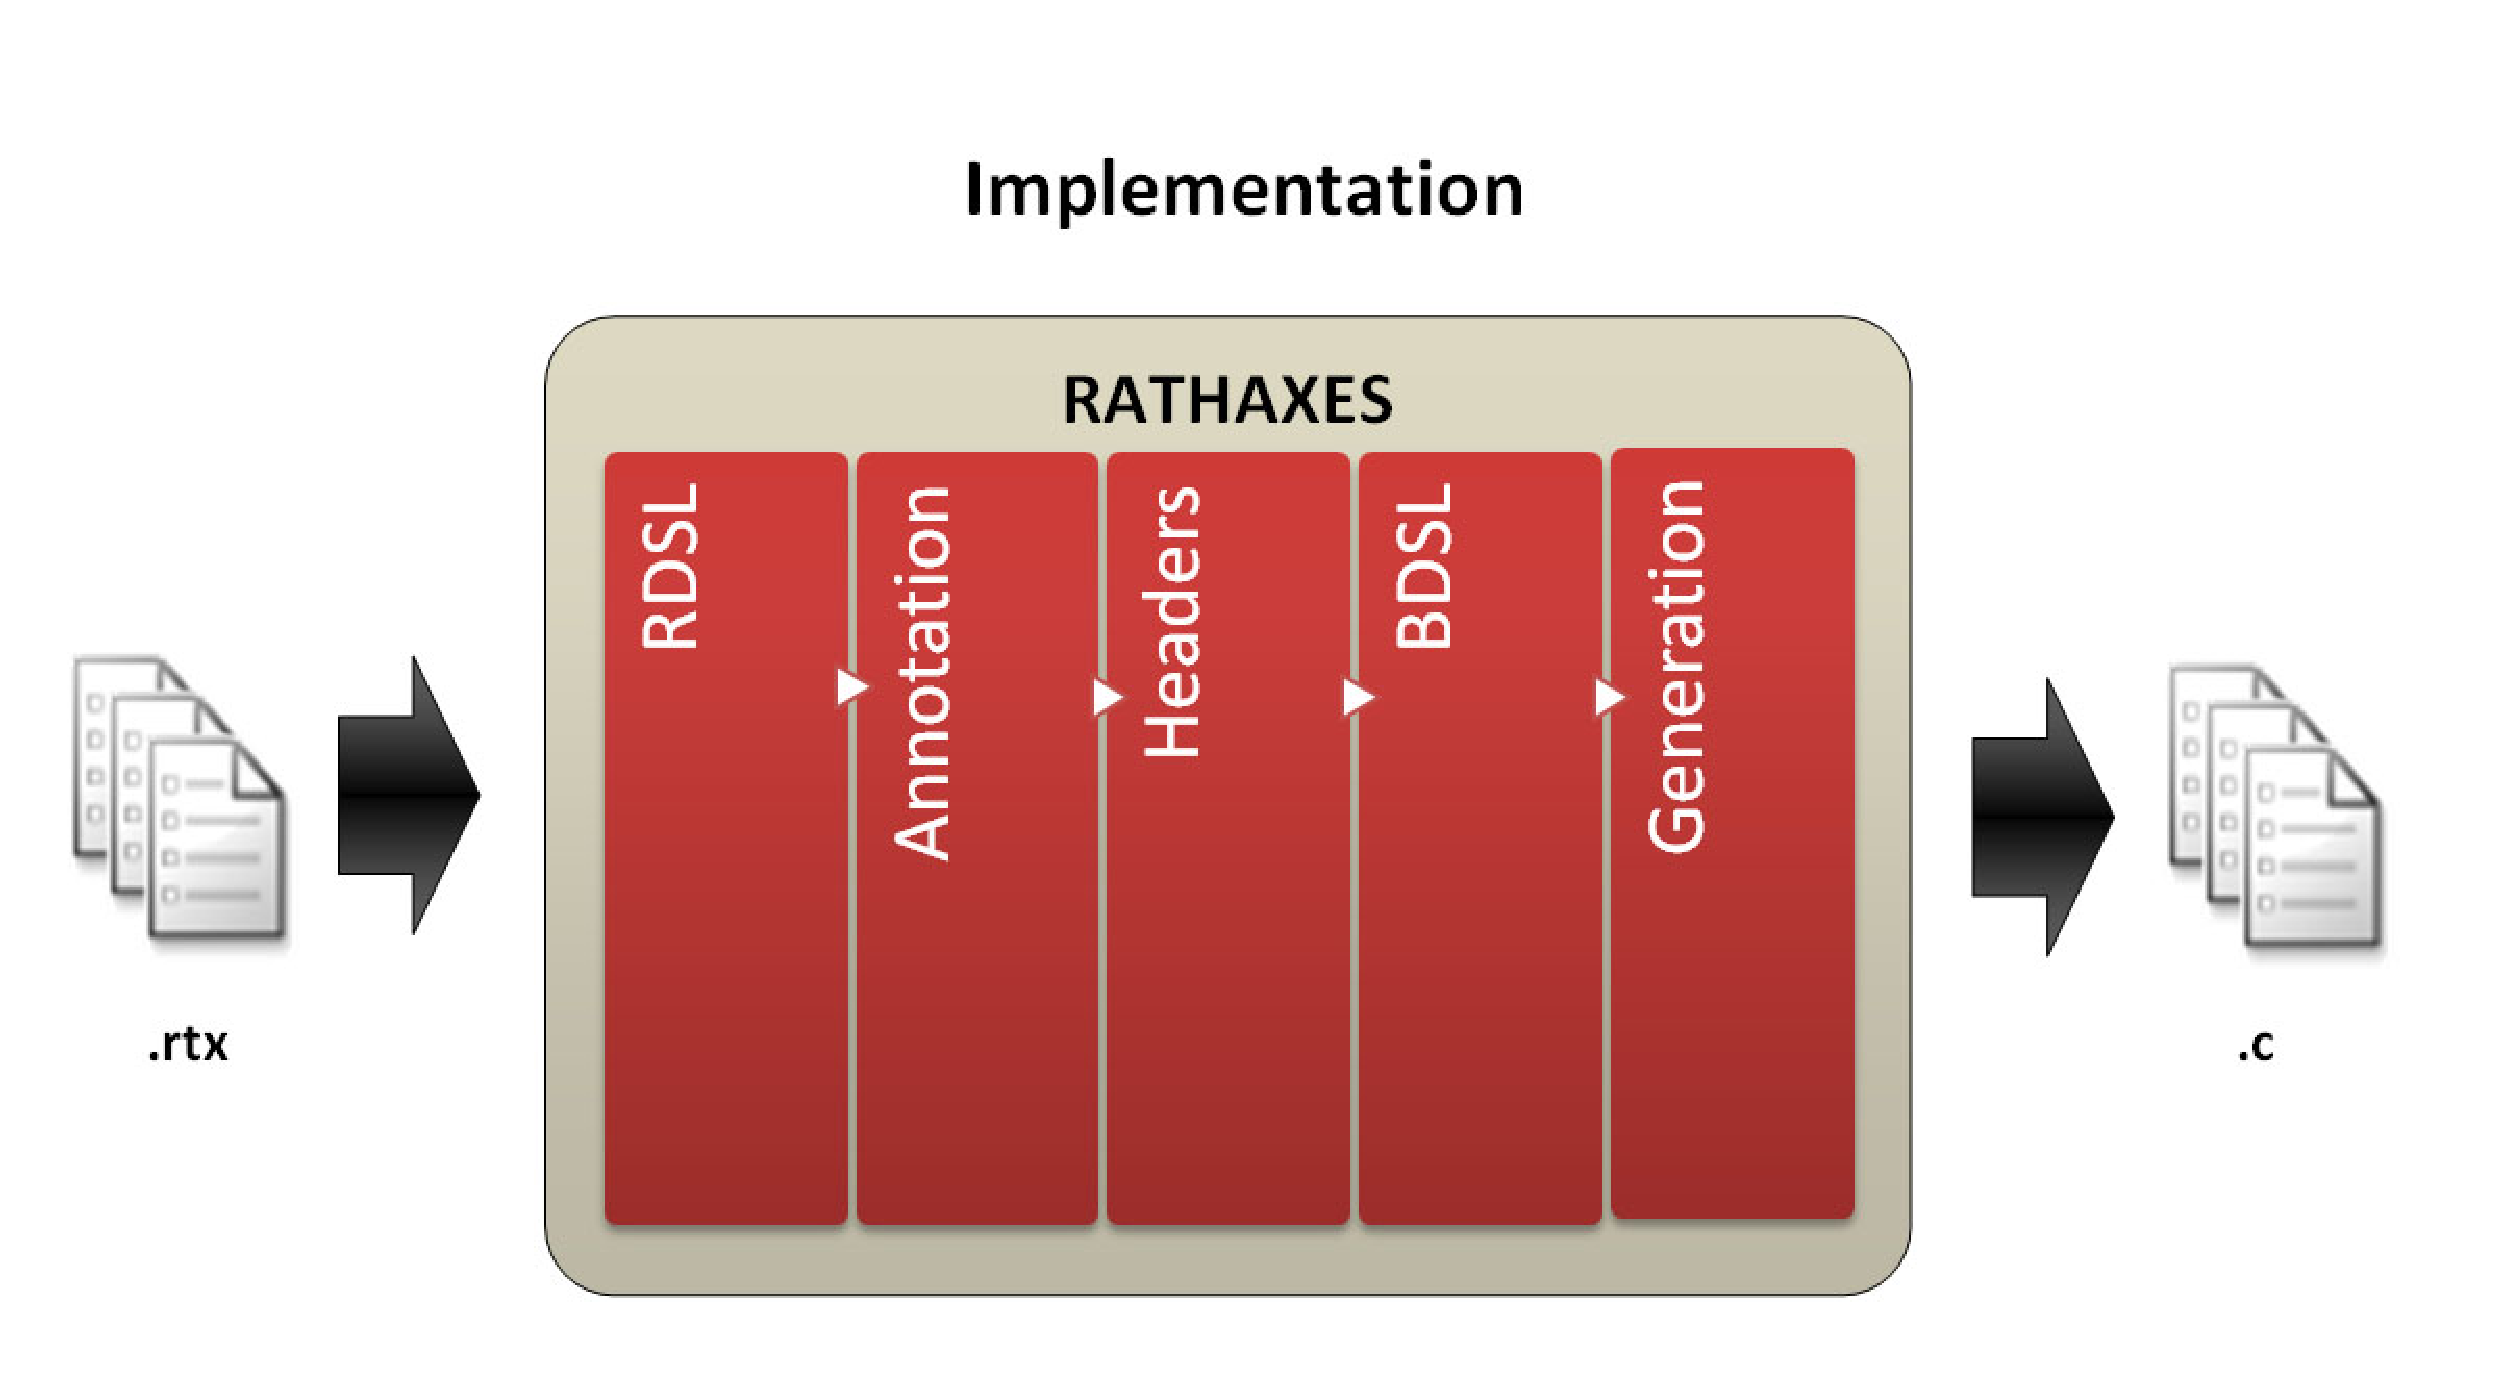
\includegraphics[width=13cm]{implementation}

    \section{RDSL parsing}
	Files of reference : rathaxes/language/rtx/scripts/parsing/rdsl\_*\\
                
	Rathaxes source files dedicated to parsing the Frontal language are all to be filed inside the "/rdsl" directory
	All the files inside this directory are meant to allow us to translate the source code, into an abstract
	syntax tree exploitable by the compiler. The rathaxes source files are all normalised according to their 
	functions. files dedicated to describing a parsing grammar are to be labeled cwp or cwh (header) according to 
	wether they can be called or have to be included. script files are to be labelled likewise cws or cwf (function)\\

        \subsection{Rathaxes DSL}
       	The Rathaxes DSL is composed syntaxically of three types of grammatical rules : 
        \begin{enumerate}
             \item Declarations \\
               This category of syntaxic statements are used to create macroscopic nodes
               inside our syntaxic tree. They are used to announce the existence of a 
               semantic object. For example the Register block (see code examples below) 
               is used to declare the existence of a register, same thing with the device
               block, driver block and userland block.
            \begin{itemize}
              \item device
 \begin{lstlisting}

DEVICE my_device
{
...
Many other declarations
...
};
\end{lstlisting}
              \item driver
                \begin{lstlisting}
DRIVER my_device ON linux
{
        TYPE = chardev;
        MAJOR = -1;
};

                \end{lstlisting}
              \item USERLAND
                \begin{lstlisting}
USERLAND
{
                SYLL open
                {
                };
                SYLL close
                {
                };
};

                 \end{lstlisting}
              \item registers
          Rathaxes was inspired bu the thesis of Mr. Laurent Reveillere, who invented the concept of
          abstracting the access of registers. There is a redundancy of information on the number
                      of bits, it is voluntary for error detection's sake.
                     We access the inner values of the registers through symbolic variables, which abstract the necessary
                     communication and stockage issues from the developpers, in this block  we will stock all the
                        relevant informations of these variables.
               \lstset{language=rathaxes}
               \begin{lstlisting}
        REGISTER my_reg[8] ON read LIKE (10...*..)
        {
                [3..5] AS configuration
                {
                        (000) -> DISABLED;
                        (001) -> ENABLE_PROPRIETY_1;
                        (010) -> ENABLE_PROPRIETY_2;
                        (101) -> RESET;
                };

                [1] AS reg_x_state
                {
                        (0) -> FALSE;
                        (1) -> TRUE;
                };

                [0] AS error
                {
                        (0) -> FALSE;
                        (1) -> TRUE;
                };
        } SET { configuration.DISABLED, reg_x_state.TRUE };
               \end{lstlisting}
         This code declares an 8 bit register, named my\_reg, that is Read only whose bits are defined thus :
         The first bit is always 1. The second bit is always 0. The third to fifth bit are meaningful and will
         have to be encapsulated inside a variable for access. The sixth bit is meaningless. \\
         just to sum up : \\
            \* : meaningless bit\\
            . : the bit is meaningful, and as such will have to  be encapsulated inside a variable during the
                implementation of the register\\
            0 : must be 0\\
            1 : must be 1\\
         \\
         Ok we're done talking about the preliminary declaration. Let's turn to the large blob of code under that
         encapsulates the variables. The value of the registers is abstracted from the developpers through these
         variables. The developper will now always have to use these variables to control his register.
         For example the third to fifth bit of the register have been defined as being ``configuration'' 
         to access these bits you\'ll have to write something like : ``my\_reg->configuration = DISABLED''\\
         that would mean that we want to set the 3 -5 bits to 000\\
         The last block Set indicates how the driver will have to set the register at initialisation of the driver.\\

         
             \end{itemize}
               
           \item Statements\\
             This category of syntaxic expressions is used to fill up the nodes we have instanciated with declarations
           \item Expressions\\
             This sub category of statements is used to edit the nodes in different cases
             \end{enumerate}
       \subsection{Abstract Syntaxic tree}
	After parsing our data is stocked inside an abstract syntaxic tree. This is the intermediate language of 
	our compiler. Its structure is documented here.\\
        \begin{lstlisting}
- The project node
 All of the data is inside the node project, in codeworker the `` this'' node.
  -- The references node
  In this node we will find various data links that will refer to the rest of the compilation context. 
  Other data meant to ease compiling and data treatment. In the long run these will be hidden behind 
  an API for the developpers.
      --- treeFile
      The file path where the tree will be saved at the end of the parsing.
      --- outputFile
      The file path where the c code will be outputted at the end;
      --- device
      Which device are we actually implementing now.
      --- driver
      the corresponding driver
      --- operatingSystem (sur lequel tu generes)
      The OS we are generating to.
  -- The devices (liste des devices decris, tableau des 7 semantics key(name) value(on/off))\\
  This node, will contain an associative array of boolean flags, with 7 entries, one for every driver 
  semantic. The flags will be activated according to wether the corresponding semantics is specified
  during parsing. The key to these entries is the name of the semantics Inside these entries we will stock
  the source data relative to that semantic node.
  It will also contain the list of the different devices
      +--- RKM
         +---- Generic information table
      +--- userland
         +---- tableau des entry points userland declares
      --- ...
      --- io
         ---- tableau des registres declares
      --- Registers 
         ----definition
         A Rathaxes Register is defined by many parameters they are stocked inside the tree by their name.
         ---- name
         The name of the register that will be used inside the RDSL to call the register
         ---- size
         the size of the register in bits. 
         ---- mode (r/w/rw)
         The access mode of the whole register. Read only for data that is meant to be read. Write only,
`	 and Read/Write
         ---- shape (***.001.)
         In this field we will stock the accessibility of the different bits of the register.
     --- tableau des variables
      The variables mapped inside the registers of the device.
          ---- definition
            ----- name
            the name of the variable a valid c identifier
            ----- range
            The bit range, from bit number so to so.
            ----- size 
            the number of bits of the variable (once again the redundancy is willful)
      --- block
      table key(valeur BINAIRE des bits) value(idendifiant associe)
      The bit value and its associated identifier.
         ---- set
         the value we should set the register to, at first execution.
                END OF SAMPLE REGISTER BLOCK
   -- driver
   A list of the drivers to generate on each os in the Rathaxes execution
\end{lstlisting}
    \section{System headers handling}
    File of reference : rathaxes/language/rtx/scripts/core/headers\_handler.cws\\
    
    For correct compilation of C code, all data type must be specifically defined
    in each compilation units. The kernel types are usually defined in the relevant
    kernel headers. A rathaxes generated driver is supposed to be robust and complete
    therefore it should only include the kernel headers it absolutely need to compile
    no more no less. We have defined a syntax in our RDSL to specify that a specific driver
    semantic requires a specific include. If the semantic is activated the header will 
    be included.\\
    A very important issue in header handling, on certain Operating Systems (Yes we're
    talking about you OpenBSD) is the order of inclusion. Because on these OSs, it is
    forbidden by the kernel coding style to include files, inside include files. Thus
    some .h files must be included before others. We have developped the following syntax
    to code that information.\\
    example : linux/dependancies.blt
\begin{lstlisting}


DEPENDENCY RKM
{
  REQUIRE linux/module.h;
  REQUIRE linux/init.h;
};

DEPENDENCY user_interface
{
  REQUIRE linux/fs.h;
  REQUIRE linux/kernel.h;
  REQUIRE linux/cdev.h
    {
      linux/types.h;
    };
};

\end{lstlisting}    

    As we've said earlier, the C code in our templates is parsed and turned into a tree
    We need to know the system types for that to work. If we were stupid that would require 
    parsing every kernel header file just to collect the system types. We tried that, 
    brought compilation time over ten minutes on windows. So we've invented a system
    of cache, which stocks the system types into a hash table to guarantee their existence.\\

    File of reference : language/rtx/black\_library/tools/parseHeaderFile.cwf \\
    
    The data is stocked inside the Bdsl tree (yeah there is only one tree, but don\'t let 
    that confuse you) thus :\\

\begin{lstlisting}
 +driver
 The driver node
   +-advices
   The advices node
     ---types 
     A list of types, with their names as key of the associative array
\end{lstlisting}

    \section{BDSL parsing}
    Reference files : rathaxes/language/rtx/scripts/parsing/bdsl*\\
    Now we'll turn our attentions to the black library, Our template repository. It is very important to understand
    that we have three different languages in them. Just look.

\begin{lstlisting}
<%

/*
**      _kernel_registration.blt in black_library/linux/RKM/
**      for Rathaxes project
**      made by Thor
*/

local   sDeviceName = this[``RKM''][``NAME''];
%>

ADVICE kernel_registration PART_OF RKM
{
  module_init(@sDeviceName@_init);
  module_exit(@sDeviceName@_exit);
};
\end{lstlisting}

    First of all we have CodeWorker, in Generation mode. What that means is that you can escape
    code and call script functions, or summon variables for generation purpose. Don't count 
    too much on it though, we're working on a script language inside the Meta and aspectual DSL
    that will replace it. But for the moment it's useful.
    You can access lots of useful informations inside the ``this.references'' Just look in the
    description of the tree a little further on.\\
    Second we've got our Meta-Aspectual DSL. Right now we only have a partial implementation.
    Only the most necessary aspects are available for the moment. that is to say the ``ADVICE''
    ,``JOINPOINT'' and ``PART\_OF'' keywords.\\
    Third we've got C, hurray at last something meaningful. That's our templates and the code
    that will be generated \\

%	/* comprends pas parfaitement difficile de parler d'implementationq quand �a n'existe pas encore */
%	* introduction de META STATEMENT (META IF, META WHILE ...)
%        * introduction de variable de contexte meta, accessible par exemple via une pseudo variable ``this'', permettant de definir des meta expressions
%        ---> il faudra definir l'interface des methodes/proprietes accessible via this pour fournir une abstraction adequate au developpeur de BLT
%        afin qu'il accede aux noeuds de l'arbre de maniere implicite et transparente.
 %       ---> ces meta expressions seront les expressions des meta statements.
%	- JOINPOINTS, aspectualisation, division des machins et l arbre a decrire
        
	We use a stabilisation based algorithm to test if all of the joinpoints have been expanded, that is to say, 
	we expand all of the node we find, and test if any of them need to be re expanded, if the system is stable 
	we stop, but if we can keep going we can stop.\\

	The parsing of the BDSL generates an abstract syntax tree, this is its structure :\\

\begin{lstlisting}
 - project
 The project node it contains everything
   -- references
   A list of different data links that will ease compilation
      --- BLTFileList
      List of all the blts that will be called upon during compilation.
      --- currentBLTFile
      The path of the current blt that we are parsing at the moment, 0 if not applicable
      --- joinpoints 
      Reference array towards all the joinpoints
      --- advices
      reference array towards all of the advices.
   -- driver
   A list of drivers, in each of these block we find the following contents.
     -- ``os''
     The name of the OS the templates are referring to.
       --- advice
         ---- Advice Array
         A simple list of all the advices of the code
           ----- table (\_C\_CODE\_) -> C code bloc | (\_JOINPOINT\_) -> point de jointure
           AS the structure of the tree so clearly explains, these nodes can be either C 
           code (Parsed as we've so often repeated by the Cnorm tool) Look inside the Cnorm
           documentation to see how it is stocked, but don't worry too much about it, 
           the generation will be done through an external tool too for these parts
           you shouldn't have to tweak it too much.
           The alternative is to find a JOINPOINT block, meaning a conditional branch of the
           compiler dependant on the semantic flags raised at compilation time. 
           these nodes have two subnodes, just look :
                ------ advice
                The name of the advice desired by the joinpoint
                ------ selected (TRUE|FALSE)
                Wether or not the Joinpoint is activated.
       
     -- BLTFiles
     A list of all the BLTfiles, whose keys are the name of the files.
     The machine indepandant BLTs,(io and algos) shall be furnished and certified by Rathaxes  

\end{lstlisting}

    \section{Aspect selection (linkage)}
    Reference File : rathaxes/language/rtx/scripts/core/aspectSelector.cws \\
	We have built the two trees sepcified higher, and we have to fuse them,
        so that they will become a more direct representation of the output file.
        Then the generation will become a more straightforward process.
        We are going to first resolve the links between these two data structures, 
        bringing to correspondance the joinpoints and their corresponding advices.
	the following scripts are dedicated to this : 
	We use the reference list as much as posssible for this step.
        . project
          . references
            . entryPoint 

        Every symbolic link in the tree of an aspect will be replaced by the selected
        aspect, and in turn it will be replaced by the C code nodes.

    \section{Generation}
    Reference File : rathaxes/language/rtx/scripts/generation/*\\

        First of all thank you for going so far in this gruesome attempt at a documentation
        We've only got one more step before the final driver file is generated, an iterative based
        run of the tree, from the beginning of the file to the end of it.
    
        GRAPH GOES HERE.

        The tool used to generate the code is called the pretty printer, it is an outside tool we
        took from Cnorm, its documentation can be found in the annexes.
	- PRETTY PRINTER -> C
          - iterBase -> selection de joinpoints, deferencement, ...
            - iterDeclaration
            - iterStatements
            - iterExpressions
	- Description de l'arbre de Cnorm
 \chapter{Annexes}
   
   \section{glossary}
    
   \section{Cnorm}

\end{document}
